\chapter{Technology} 

Many technologies were looked into and experimented with. Then the positives and
negatives of each option was weighed up before a decision was made about which would be the
suitable choice for the visualisation. It came down to 3 potential technologies that
would be suitable for the project, the next 3 subsections outline these in
detail.

\subsection{Processing}
Processing is an open source programming language and development environment
that was initially created to serve as a software
sketchbook and to teach the fundamentals of computer programming with a visual
context.
Using processing would mean that the visualization could be built with Java
while still using
a successful visualisation framework. The most complete existing visualization
using
the same exoplanet dataset (Kepler Visualization Tool) is built using
Processing.
Using this solution would involve learning the Processing language, however
Processing
is a library built in Java so the syntax is the same. This means the learning
curve should be shallow.
Using processing means that 3D elements could be included, this wouldn't be
possible with D3.

\subsection{D3 (Data Driven Documents)}
D3 is a JavaScript library that allows the displaying of data in dynamic
graphics. Embedded
within an HTML web page, the JavaScript D3.js library uses pre-built JavaScript
functions to
select elements, create Scalable Vector Graphic (SVG)[17] objects, style them,
and add transitions,
dynamic effects and tooltips. Large datasets can be easily bound to SVG objects
using
simple D3 functions to generate rich charts and diagrams. D3 was created because
of the
need for a balance of expressiveness, efficiency, and accessibility that
previous visualization
toolkits did not allow [4].

D3 allows the binding of input data to arbitrary input elements. This means that
the exoplanet dataset can easily be bound to SVG elements for creating visualizations. D3
adopts the W3C Selectors API to identify document elements queried. This results in a
rich but concise selection method of elements in a visualisation. It allows debugging thanks to Google chrome and other modern browsers
development tools. A downside to D3 is that it does not allow 3D diagrams, although it does
allow pseudo 3D by using the painters algorithm and 3D textures.

\subsection{Prefuse}
Prefuse is a set of software tools for creating rich interactive data
visualizations [13]. The
Prefuse toolkit provides a visualization framework for Java. It supports a set
of features
for visualizing and interacting with data. It provides optimized data structures
for tables,
graphs, and trees. It can be used to build standalone applications, visual
components embedded
in larger applications, and web applets. Prefuse to greatly simplifies the
process
of representing and efficiently handling data, mapping data to visual
representations (e.g.,
through spatial position, size, shape, color, etc), and interacting with the
data.
To use Prefuse a basic familiarity with the Java is required, including setting
up and building
Java projects. A knowledge of Swing or another similar user interface toolkit is
also
useful for understanding some of the concepts behind Prefuse and for integrating
Prefuse
visualizations into larger applications. Experience with database systems is
also helpful. 
However the complexity of Prefuse means that the learning curve will be out of
scope for
this project.


\subsection{Decision of technology}
The final decision of technology was to use Processing, this is because it had
many positive aspects that the others did not and minimal negatives as the below
table illustrates.
\clearpage
\begin{figure}[H]
  \centering
      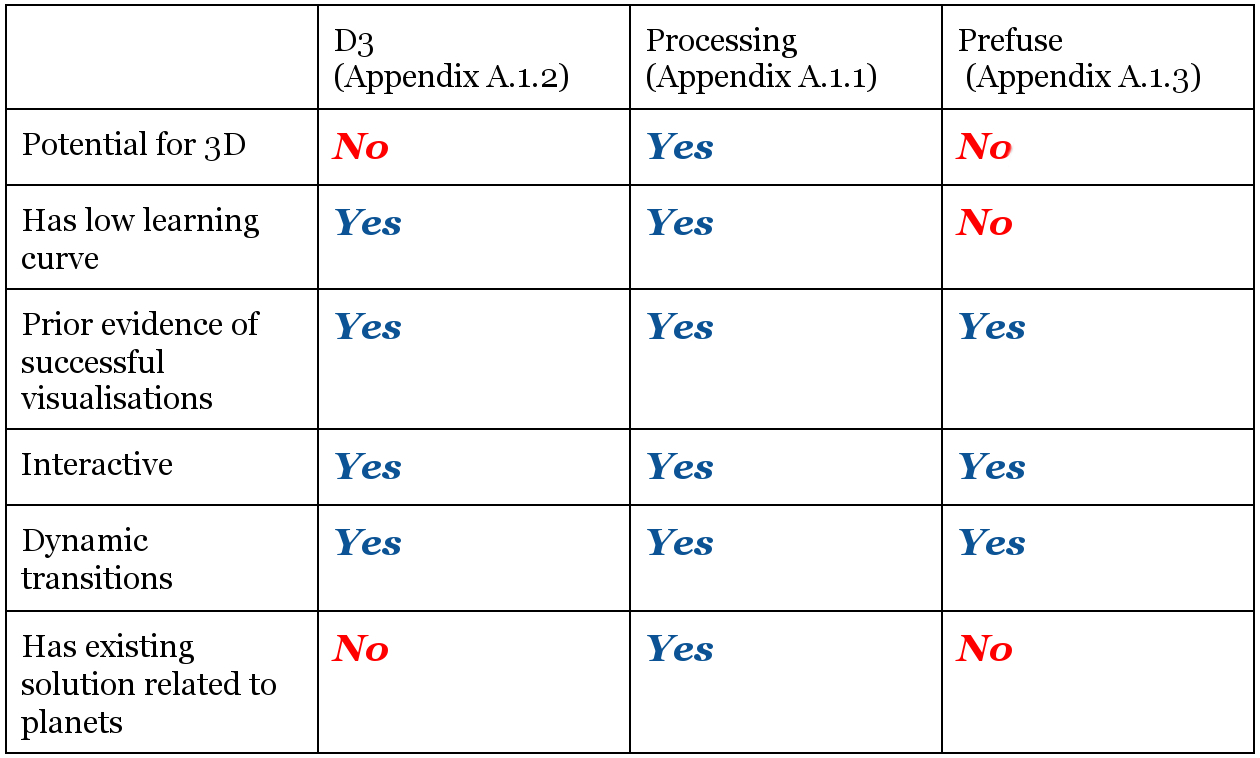
\includegraphics[width=0.8\textwidth]{images/table_technologies.jpg}
  \caption{Table of technology choices}
\end{figure}

As this project was created using Processing, it allowed me to extend the
previous visualisation using the same data set, The Kepler Visualisation Tool
\cite{kepler_github, kepler_article}. As the time was short for this project
building upon a previous solution increased the amount of progress that could be
made in the time afforded.

Taking this approach meant that the languages being used would be Java using
processing libraries. 

As this is such a large project involving many different iterations, version
control was important for maintaining records and backups of important changes
which was stored on remote servers to ensure against file loss in system
failures.

